% Publication-quality diagram for separate neural network model

\documentclass{article}
\usepackage[margin=0.5in]{geometry}
\usepackage{tikz}
\usetikzlibrary{shapes.geometric, arrows.meta, positioning}
\pagestyle{empty}

\definecolor{inputblue}{RGB}{102,194,255}
\definecolor{processorange}{RGB}{255,179,102}
\definecolor{probgreen}{RGB}{153,221,153}
\definecolor{outputyellow}{RGB}{255,255,153}
\definecolor{backpropred}{RGB}{220,50,47}

\begin{document}
% Add a small manual vspace above and below, and hspace left/right using a tikz "scope" with shift
\vspace*{1em}
\noindent
\hspace*{1em}%
\sffamily
\textbf{\fontsize{16}{18}\selectfont Separate Neural Networks Architecture}
\vspace{0.5em}

\begin{center}
\setlength{\abovedisplayskip}{0pt}
\setlength{\belowdisplayskip}{0pt}
\setlength{\abovedisplayshortskip}{0pt}
\setlength{\belowdisplayshortskip}{0pt}
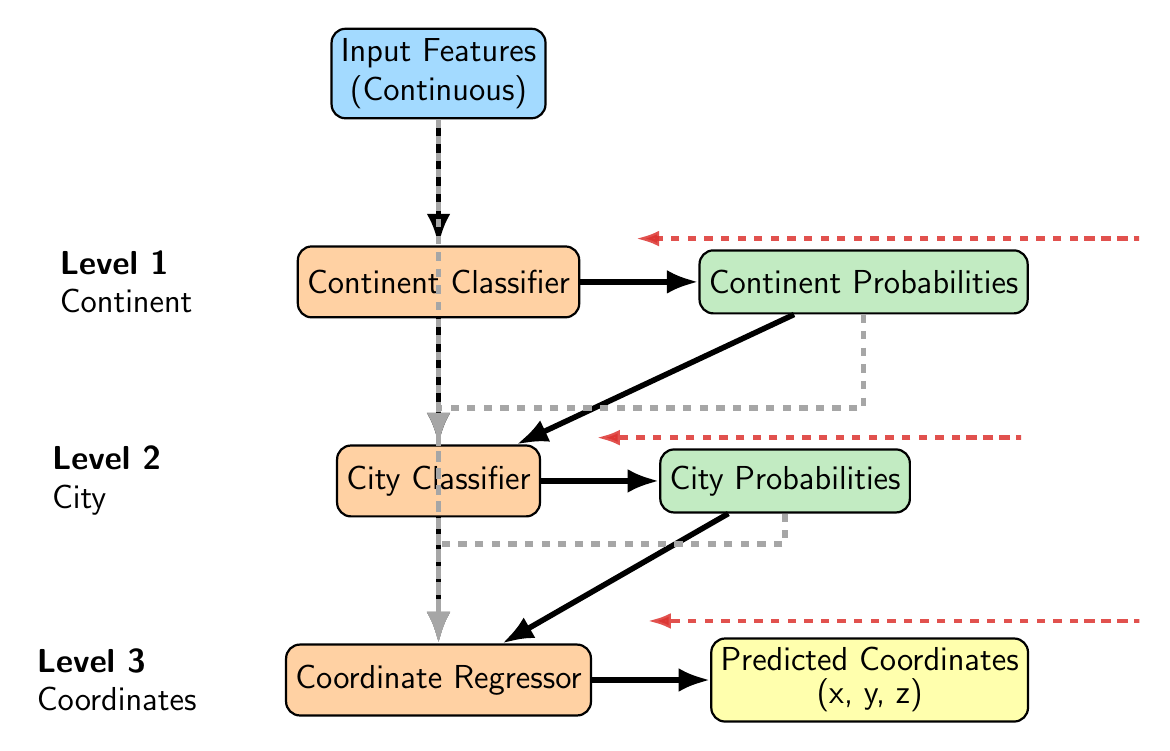
\begin{tikzpicture}[xshift=10, yshift=10,
    node distance=1.6cm and 1.8cm,
    every node/.style={font=\sffamily\large},
    input/.style={rectangle, rounded corners=5pt, draw=black, fill=inputblue!60, minimum width=2.2cm, minimum height=0.9cm, thick},
    process/.style={rectangle, rounded corners=5pt, draw=black, fill=processorange!60, minimum width=2.5cm, minimum height=0.9cm, thick},
    prob/.style={rectangle, rounded corners=5pt, draw=black, fill=probgreen!60, minimum width=2.2cm, minimum height=0.8cm, thick},
    output/.style={rectangle, rounded corners=5pt, draw=black, fill=outputyellow!80, minimum width=2.2cm, minimum height=0.9cm, thick},
    arrow/.style={very thick, -{Latex[length=4mm,width=3mm]}, line width=2pt},
    backprop/.style={ultra thick, dashed, -{Latex[length=3mm,width=2mm]}, color=backpropred, opacity=0.85},
    concat/.style={very thick, -{Latex[length=4mm,width=3mm]}, color=gray!70, dashed, line width=2pt},
    legend/.style={rectangle, draw=none, fill=none, font=\large}
]

% Nodes (compact layout)
\node[input] (input) {\shortstack{Input Features\\(Continuous)}};
\node[process, below=of input] (cont) {Continent Classifier};
\node[prob, right=1.5cm of cont] (contprob) {Continent Probabilities};

\node[process, below=of cont] (city) {City Classifier};
\node[prob, right=1.5cm of city] (cityprob) {City Probabilities};

\node[process, below=of city] (coord) {Coordinate Regressor};
\node[output, right=1.5cm of coord] (output) {\shortstack{Predicted Coordinates\\(x, y, z)}};

% Straight forward arrows
\draw[arrow] (input) -- (cont);
\draw[arrow] (cont) -- (contprob);
\draw[arrow] (cont) -- (city);
\draw[arrow] (contprob) -- (city);
\draw[arrow] (city) -- (cityprob);
\draw[arrow] (city) -- (coord);
\draw[arrow] (cityprob) -- (coord);
\draw[arrow] (coord) -- (output);

% Feature augmentation arrows (gray dashed, like combined)
\draw[concat] (input) -- ++(0,-1.6) -| (city);
\draw[concat] (input) -- ++(0,-3.2) -| (coord);
\draw[concat] (contprob) -- ++(0,-1.6) -| (coord);
\draw[concat] (cityprob) -- ++(0,-0.8) -| (coord);

% Level labels (larger font, closer to nodes)
\node[align=left, left=1.2cm of cont] (l1) {\textbf{\large Level 1}\\\large Continent};
\node[align=left, left=2.1cm of city] (l2) {\textbf{\large Level 2}\\\large City};
\node[align=left, left=1.0cm of coord] (l3) {\textbf{\large Level 3}\\\large Coordinates};

% Backpropagation arrows (local only, further above and smaller, coordinate arrow higher)
\draw[backprop] ([yshift=0.55cm,xshift=0.7cm]contprob.east) -- ++(0.7,0) |- ([xshift=0.7cm,yshift=0.55cm]cont.east);
\draw[backprop] ([yshift=0.55cm,xshift=0.7cm]cityprob.east) -- ++(0.7,0) |- ([xshift=0.7cm,yshift=0.55cm]city.east);
\draw[backprop] ([yshift=0.75cm,xshift=0.7cm]output.east) -- ++(0.7,0) |- ([xshift=0.7cm,yshift=0.75cm]coord.east);

\end{tikzpicture}

\vspace{1.5em}
\begin{minipage}{0.95\textwidth}
\centering

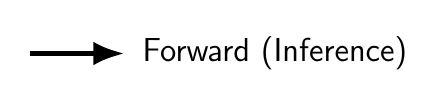
\begin{tikzpicture}[every node/.style={font=\sffamily\large}]
    \draw[very thick, -{Latex[length=4mm,width=3mm]}, line width=2pt] (0,0) -- (1.2,0); 
    \node[right] at (1.3,0) {Forward (Inference)};
\end{tikzpicture}

\vspace{0.5em}


\begin{tikzpicture}[every node/.style={font=\sffamily\large}]
    \draw[ultra thick, dashed, -{Latex[length=3mm,width=2mm]}, color=backpropred, opacity=0.85] (0,0) -- (1.2,0); 
    \node[right] at (1.3,0) {Backpropagation (local only)};
\end{tikzpicture}

\vspace{0.5em}


\begin{tikzpicture}[every node/.style={font=\sffamily\large}]
    \draw[very thick, -{Latex[length=4mm,width=3mm]}, color=gray!70, dashed, line width=2pt] (0,0) -- (1.2,0); 
    \node[right] at (1.3,0) {Feature Concatenation};
\end{tikzpicture}
\end{minipage}

\end{center}
\vspace*{1em}

\end{document}
